A significant advantage of using FastAPI is its native support for the automatic generation of interactive \acs{api} documentation. By leveraging Python type hints and the Pydantic models defined for each endpoint, FastAPI automatically creates a detailed OpenAPI specification for the entire backend.

This specification is then used to render an interactive documentation interface (Swagger \acs{ui}), available at the \texttt{/docs} endpoint. To enhance security and usability, a custom function \texttt{auth\_openapi} was implemented to inject a \acs{jwt} bearer token authentication scheme directly into the Swagger \acs{ui}, as shown in Figure~\ref{FIG:SWAGGER_AUTH}. This allows authenticated users to view their access key on the frontend and use it to test every \acs{api} endpoint directly from their browser, providing a powerful tool for debugging and development.

\begin{figure}[Swagger UI]{FIG:SWAGGER_AUTH}{Screenshot of the interactive Swagger \acs{ui} with authorization enabled.}
    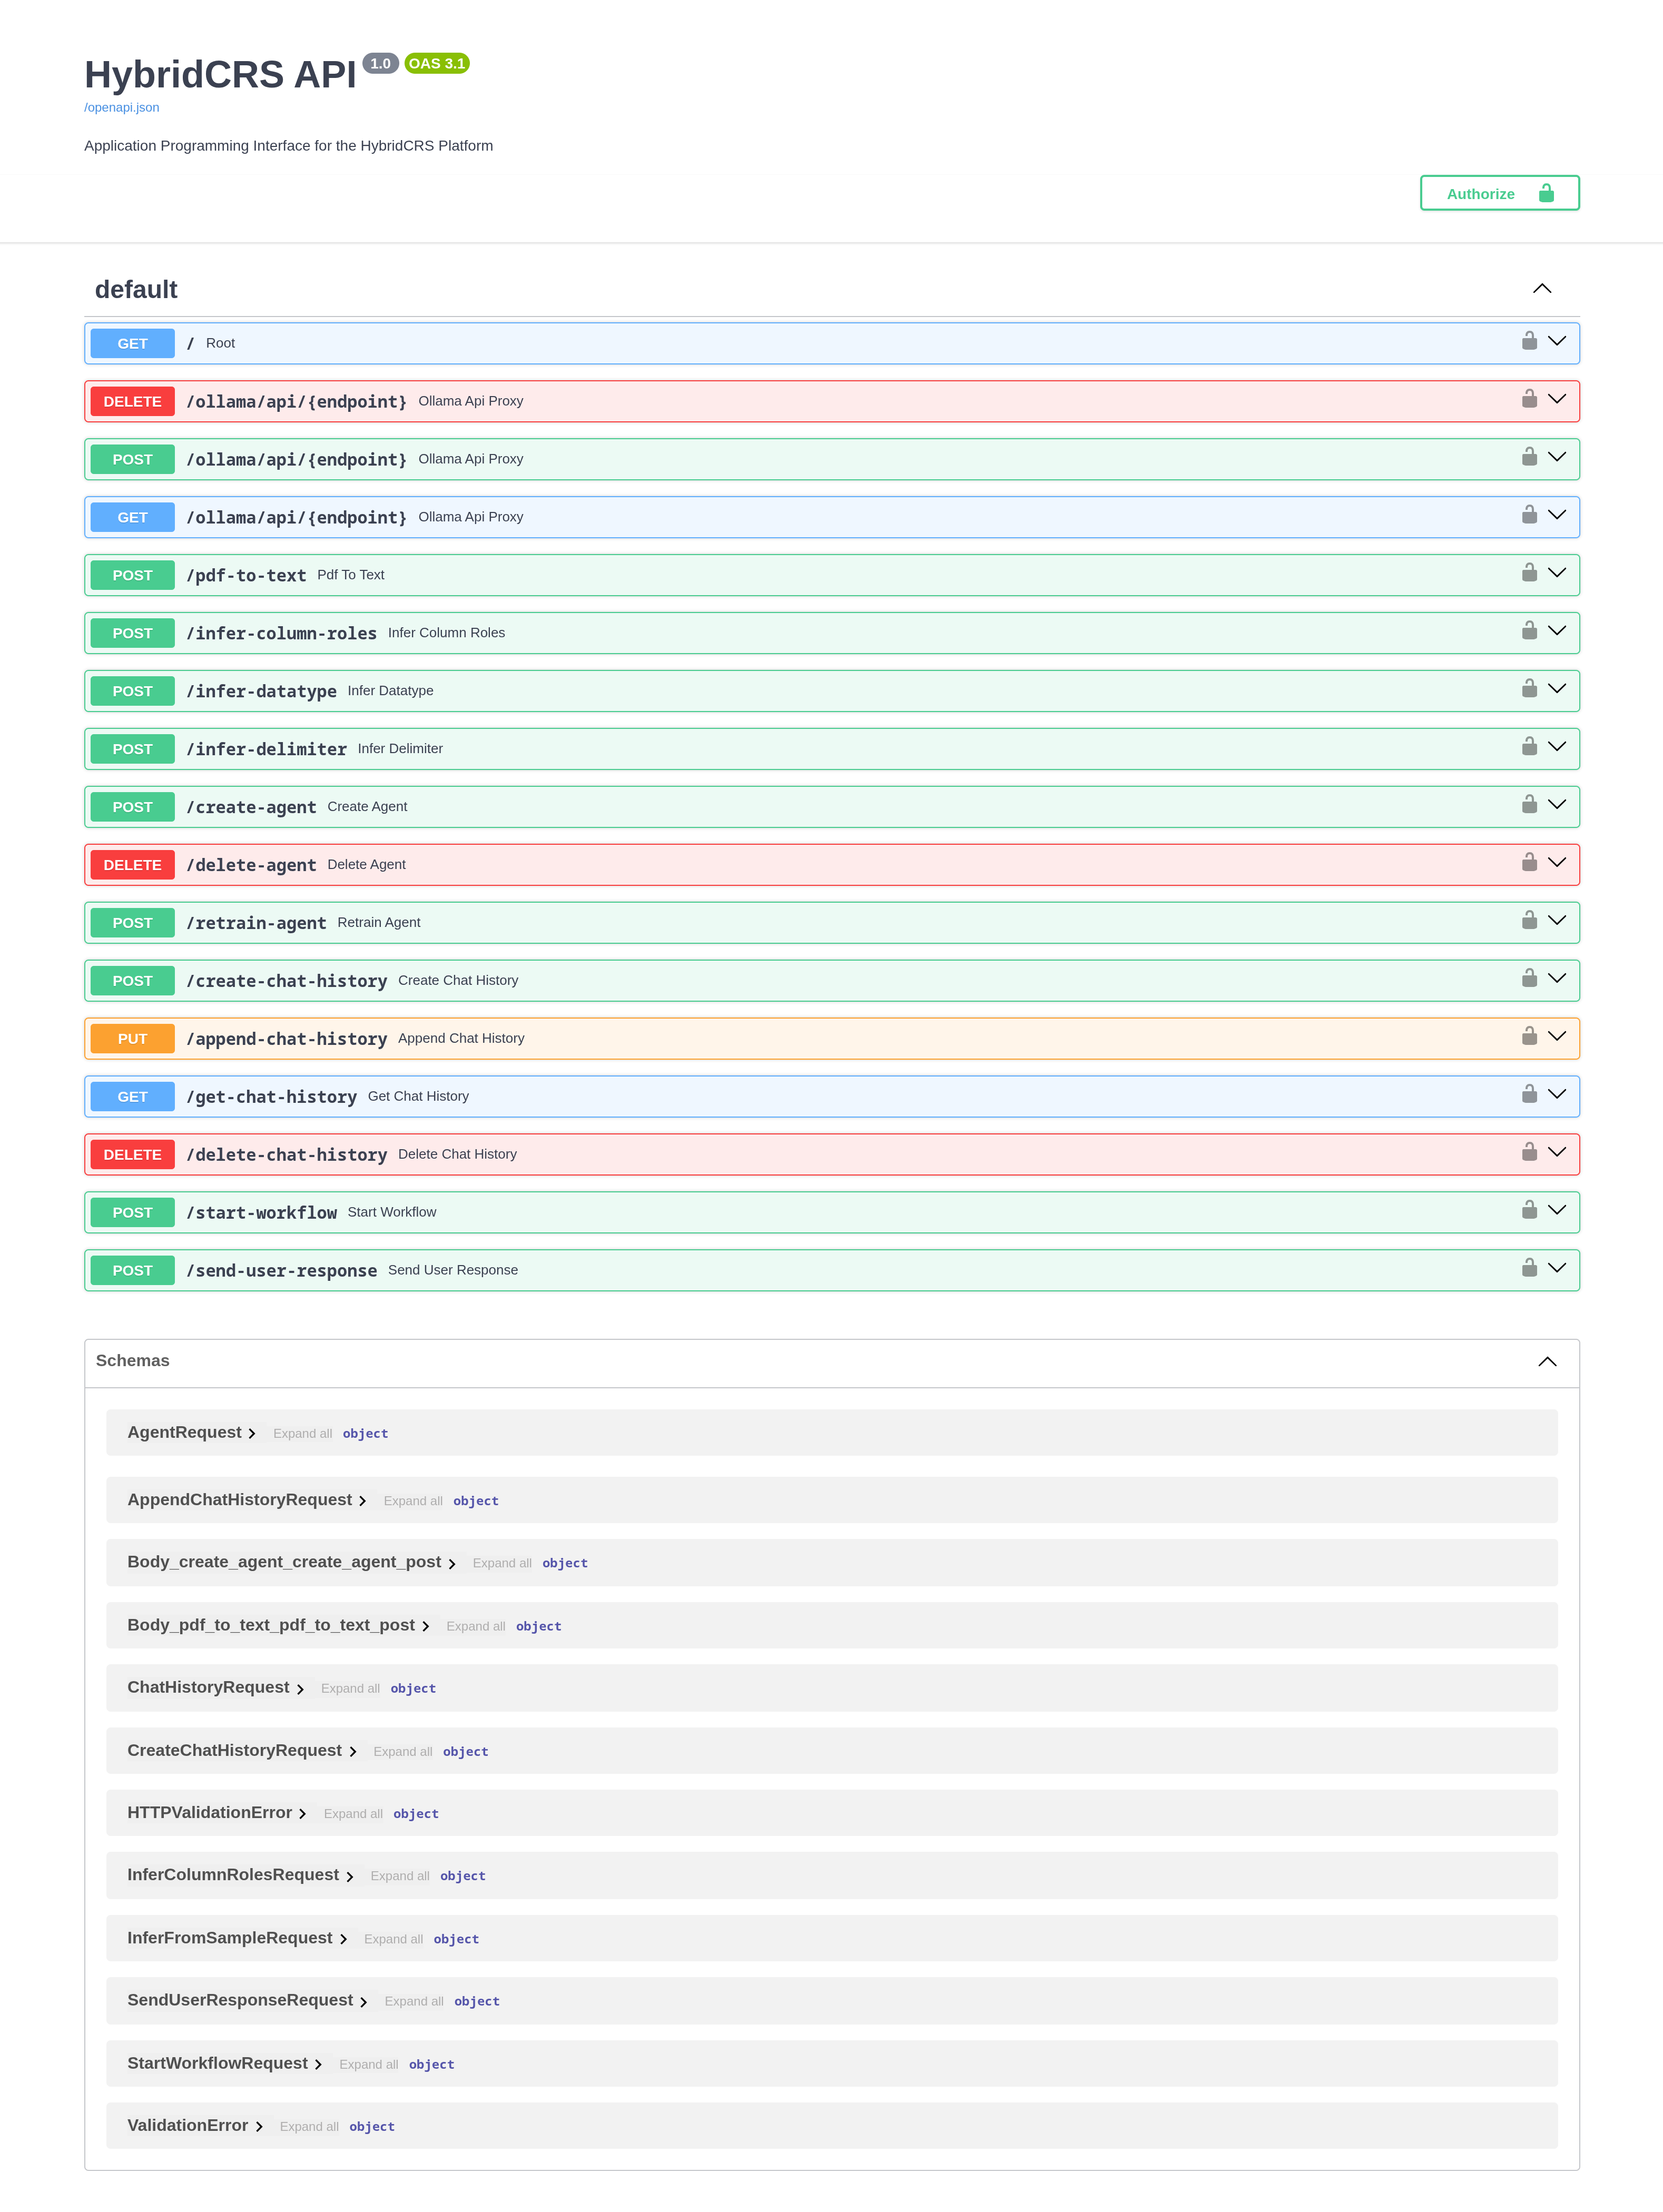
\includegraphics[width=\textwidth]{screenshots/swagger_ui.png}
\end{figure}